\documentclass[12]{beamer}

\usepackage[russian]{babel}
\usepackage{tikz}


\usetheme[progressbar=frametitle]{metropolis}
\setbeamertemplate{frame numbering}[fraction]
\usefonttheme{metropolis}
\setbeamercolor{background canvas}{bg=white}


\title{Семинар 8}
\subtitle{Эффект Зеемана. Правила отбора}
\author{}
\date{\today}
\institute {\large 
\textbf{Ключевые слова}: Эффект Зеемана, правила отбора, четность\\[6pt] 

\\[6pt] 
\textbf{Задачи}: 6.21, Т4\\[6pt] 

}


\begin{document}
\metroset{block=fill}
\maketitle


\begin{frame}[t]{Внешний одноквантовый фотоэффект}

\end{frame}

\begin{frame}[t]{Внешний одноквантовый фотоэффект}
\begin{block}{Закон Эйнштейна}
\begin{equation*}
    \hbar \omega = \dfrac{m_eV^2}{2} + A_{\text{вых}}
\end{equation*}
\end{block}
\begin{columns}[onlytextwidth]
\column{0.55\textwidth}
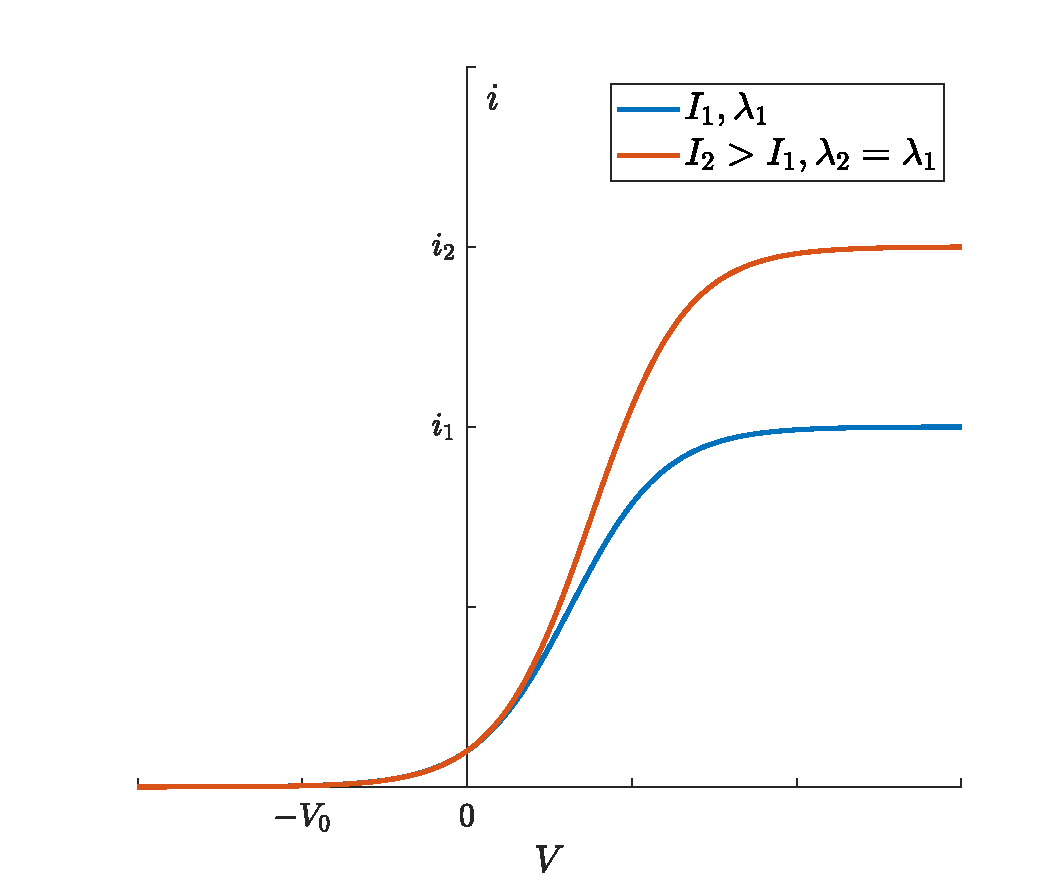
\includegraphics[width=\textwidth]{Seminar_02/pics/pic_01.pdf}
\column{0.45\textwidth}
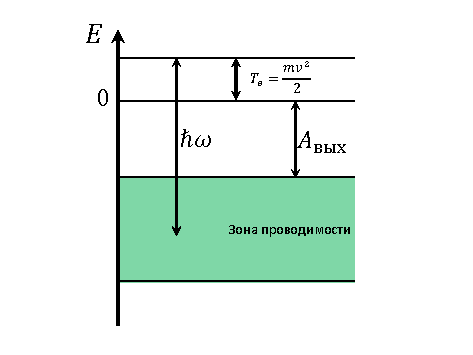
\includegraphics[width=\textwidth]{Seminar_02/pics/pic_02.pdf}
\end{columns}
\end{frame}

\begin{frame}[t]{Эффект Комптона}
\only<1>{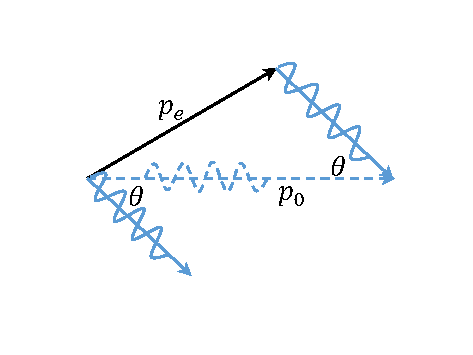
\includegraphics[width=\textwidth]{Seminar_02/pics/pic_03.pdf}}
\only<2>{}


\end{frame}




\begin{frame}{Задача }\scriptsize
\only<1>{\begin{block}{Условие}

\end{block}}
\only<2>{\begin{block}{Решение}

\end{block}}
\end{frame}

\begin{frame}{Задача }\scriptsize
\only<1>{\begin{block}{Условие}

\end{block}}
\only<2>{\begin{block}{Решение}

\end{block}}
\end{frame}

\begin{frame}{Задача }\scriptsize
\only<1>{\begin{block}{Условие}

\end{block}}
\only<2>{\begin{block}{Решение}

\end{block}}
\end{frame}

\begin{frame}{Задача }\scriptsize
\only<1>{\begin{block}{Условие}

\end{block}}
\only<2>{\begin{block}{Решение}

\end{block}}
\end{frame}

\begin{frame}{Задача }\scriptsize
\only<1>{\begin{block}{Условие}

\end{block}}
\only<2>{\begin{block}{Решение}

\end{block}}
\end{frame}



\begin{frame}[t]{Комментарии к задачам из задания}\scriptsize
\begin{itemize}
\item 
\item 
\item 
\item
\item
\item
\item
\item
\end{itemize}
\end{frame}

\end{document}